\documentclass{article}
\usepackage[utf8]{inputenc}
\usepackage{amssymb}
\usepackage{tikz}
\usepackage{amsmath}
\usepackage{relsize}
\usepackage{mathtools}
\usepackage{textcomp}
\usepackage{eurosym}
\usepackage{amssymb}
\usepackage{systeme}
\usepackage{mathtools}
\usepackage{todonotes}
\title{Results}
\author{Roman Oort}
\date{\today}

%%% PERSONAL SHORTCUTS
\DeclareMathOperator*{\plim}{plim}
\newcommand{\T}{\textbf{T}}
\newcommand{\Tij}{\textbf{T}_{ij}}
\newcommand{\Soc}{(\T(n))^{\infty}_{n=1}}
\newcommand{\beli}[3][2]{p_{#2}^{(#3)}}
\newcommand{\belvec}[2]{\textbf{p}^{(#2)}}

\begin{document}

\maketitle

\tableofcontents
\newpage
\section{Results}

All results obtained and discussed in the following section are generated with an identical network structure, unless mentioned otherwise. The networks used are all directed networks, with an increased degree, using the default distribution for the degree increase. Furthermore, the probability of a self-link is $1$, meaning that every agent will have a link to itself. Finally, uniform weight initialization was applied. Furthermore, whenever an updating rule did not lead to uniform convergence, the mean of the belief vector was taken as the convergent belief.

\newpage

\subsection{Cooperative Networks}

As can be seen in Figure \ref{coop:threshold}, in a cooperative network all updating rule behave quite similar. For smaller network sizes the convergent belief seems to differ the most between updating rules. However, as the network size increases this difference dissipates, and the convergent beliefs become more and more similar, both to the other updating rules \emph{and} the assumed truth of the model. However, while the convergent beliefs are mostly similar, the standard deviation of the convergent belief vector does differ significantly between updating rules. Where the regular and thresholded DeGroot mechanics have no deviation in the convergent belief vector, meaning they have a uniform convergent belief held by every agent, the other updating rules end up with a non-insignificant amount of variation in the belief vector. This means that, at the time of convergence, it is not the case that the different agents all hold the same beliefs, but rather, while their opinions may not change anymore, they still hold different opinions. Finally, the thresholded and regular DeGroot mechanics both reach convergence in the same amount of time, while the other updating rules are significantly faster to reach the point of convergence.

\begin{center}\todo{Fix legend}
    \begin{figure}[!htbp]
        \centering
        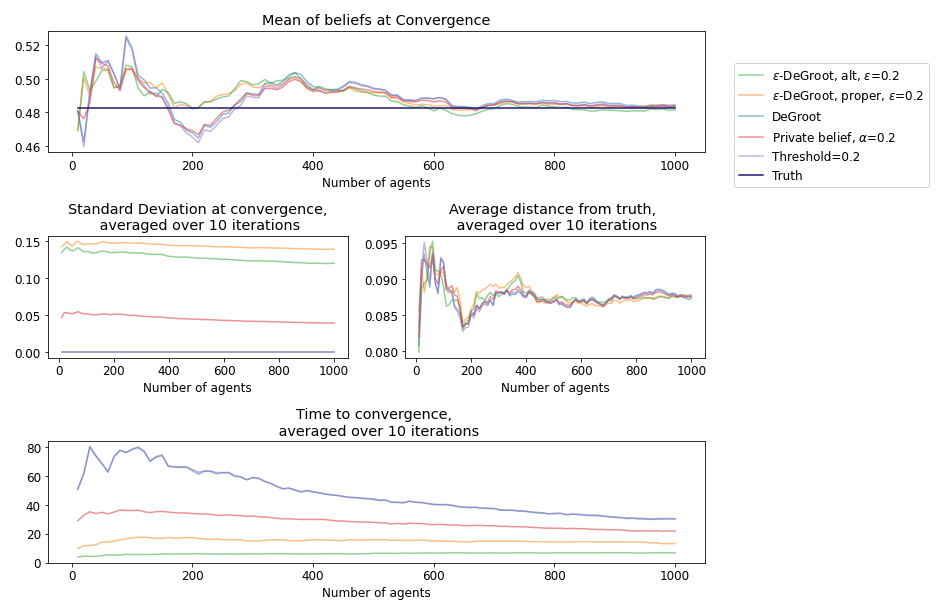
\includegraphics[width=1.2\textwidth]{ThesisKI/Images/WisdomCompare0.png}
        \caption{Convergence Behaviour Threshold Updating}
        \label{coop:threshold}
    \end{figure}
\end{center}

\subsection{Non-cooperative networks, $n=1$}

\subsection{Non-cooperative networks, $n > 1$}

\end{document}